\chapter{Risk Assessment and Mitigation}
\section{Introduction}
Throughout the project we will face a number of potential risks however we will do our best to mitigate them.
When analysing the risks we will focus on two factors, likelihood and severity.

A risk can either have a high, medium, or low chance of becoming a reality.
If a problem is not likely to occur when running a project three times or more we deem it to have a low likelihood.
If it is likely to occur once during the project or when running a project twice we deem it medium likelihood.
Finally, if it is likely to occur multiple times during the project, we will deem it as high likelihood.

A risk can also either be high, medium, or low in severity.
A high severity risk could result in months of lost progress up to having to totally start over.
A medium severity risk could result in the loss of between one week and a few weeks of progress.
Finally a low severity risk would only result in a maximum of a few days of lost progress.

To combine these two factors into something meaningful we will use a risk matrix (Figure~\ref{fig:risktable}).
This will allow us to find a balance and identify the risks that will pose major problems.

\begin{figure}[h]
	\begin{centering}
		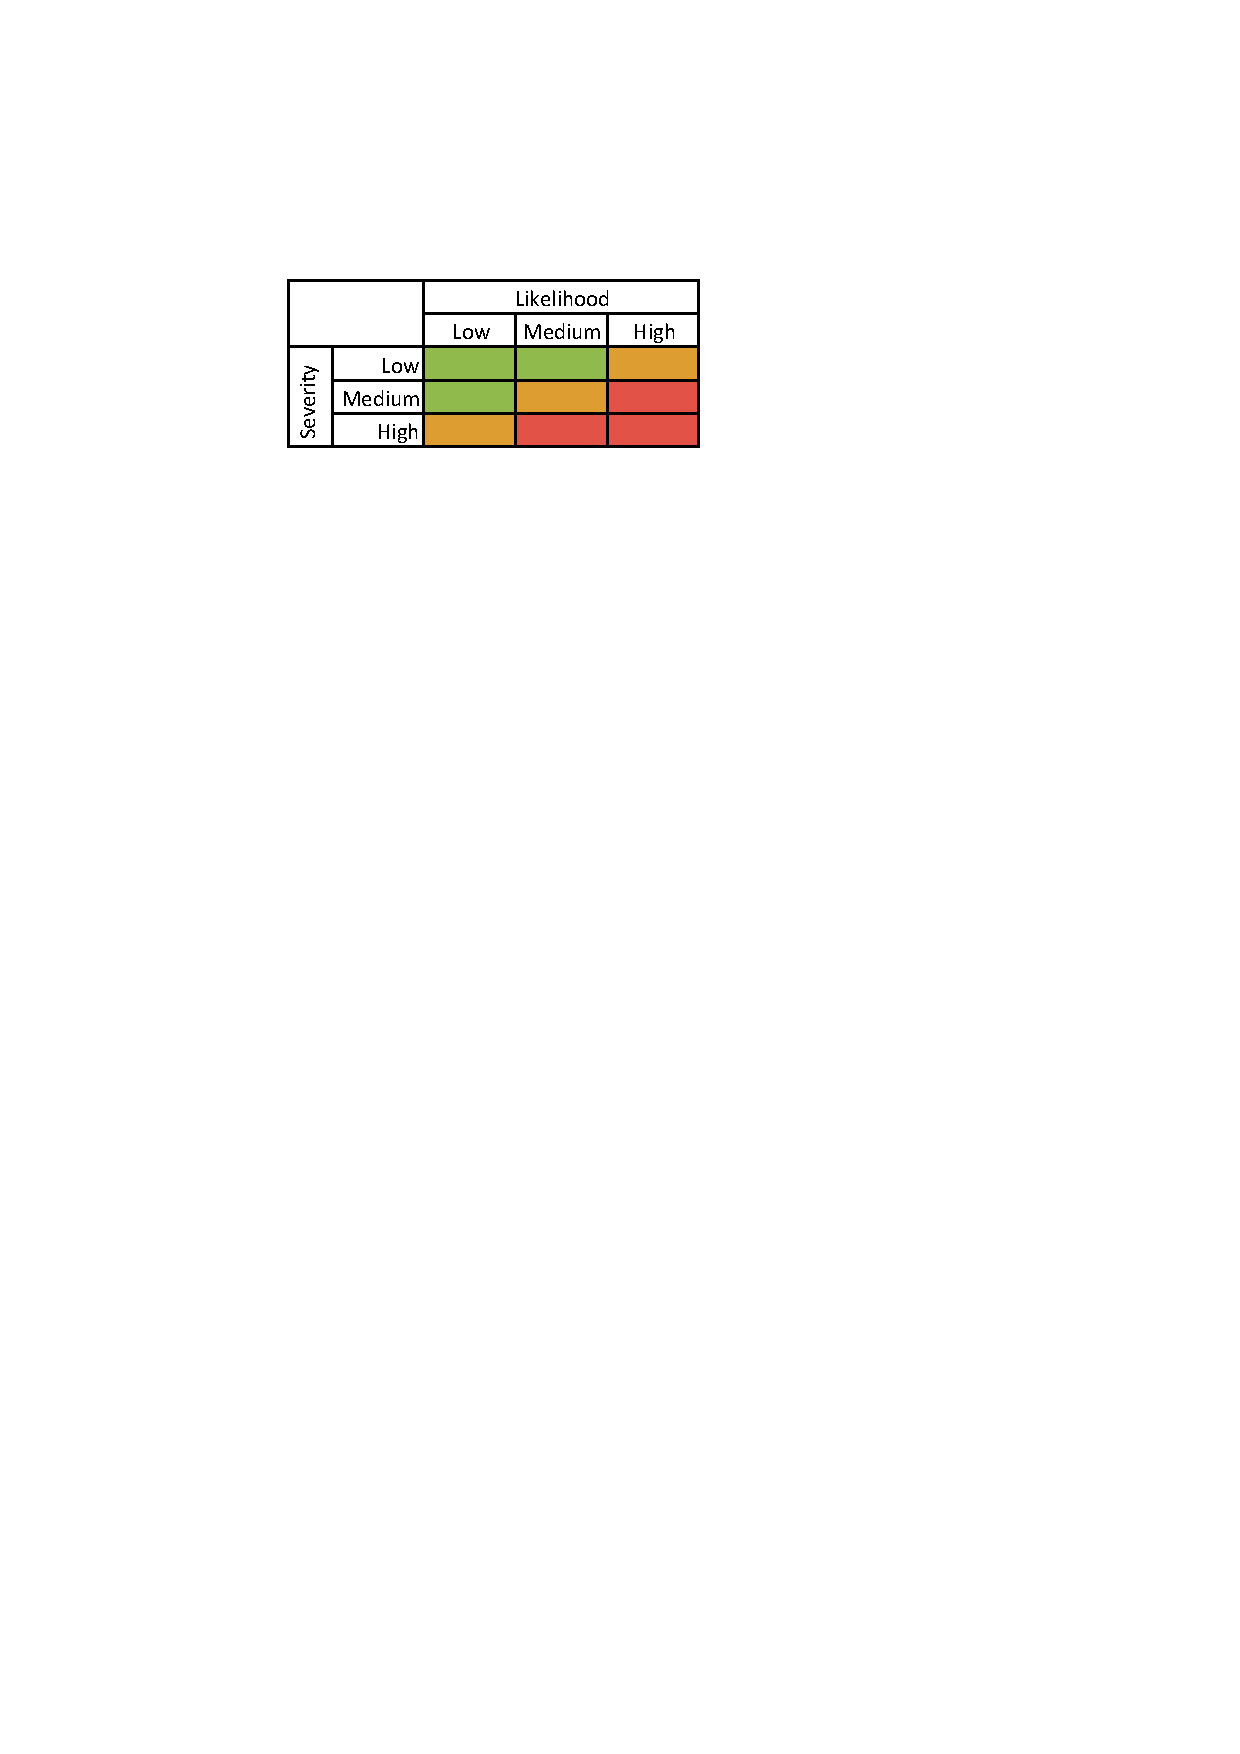
\includegraphics{risktable.pdf}
		\caption{Table showing how likelihood and severity of a risk combine to show overall impact of the risk}
		\label{fig:risktable}
	\end{centering}
\end{figure}

Green cells in the matrix are considered to be overall low risk, this is because they are not particularly likely to happen and if they do they will not have be severe enough to majorly impact the project.
Orange cells signify an overall medium risk.
They are either likely to happen but low severity, very unlikely to happen but would have a very severe impact or somewhere between.
Overall high severity risks, red cells, are the most important to mitigate.
They have a reasonably high chance of happening and could result in the loss of weeks or months of work.

It is important to categorise risks once they have been identified so that we can prioritise mitigation, it is imperative that overall high risks cannot happen and in the case that they do we must be able to cope with them and have protocols in place to lessen the impact.

We will be presenting the risks in a risk register with columns identifying, analysing and showing the mitigations for the risk.
This will give us an accessible and easily modifiable document which we will be able to use throughout the project when considering or attempting to mitigate risks.

\newpage
\section{Risk Assessment}